\begin{abstract}
Zero-cost NAS proxies rank architectures from a single pass at initialization,
yet a score that ranks with accuracy in one setting can rank against it in
another. Using a 29-feature zoo on the topology and size axes of NAS-Bench-201,
we observationally separate a dominant capacity-associated factor from an
early-trainability residual. The factor explains $52.9\%/49.4\%$ of zoo
variation and remains associated with effective rank under raw/global
orientation, but the cross-axis loading cosine falls from $0.87$ under
outcome-informed orientation to $0.46$. Several raw proxies also reverse sign,
including the condition-number sum ($+0.88\,{\to}\,-0.77$); dimension and
matched-sample controls support
a dimension-linked/proxy-geometry-dependent failure, not an independent
mechanism, while matched-sample-count resampling preserves the headline reversals. Two
controlled search traps incur $+5.40$ and $+1.97$ point costs at $K{=}10$, while
two null directions incur zero. The diagnostic uses cached target-calibration
labels and is not fully label-free. These benchmark-bound results motivate
validating proxy orientation before transporting a source ranking.
\end{abstract}

\begin{figure}[t]
  \centering
  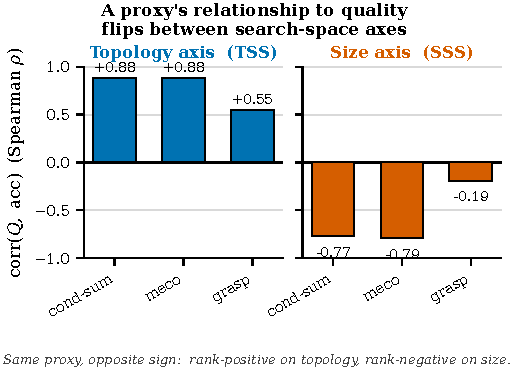
\includegraphics[width=\linewidth]{figures/fig1_signflip.pdf}
  \caption{\textbf{The cross-space sign-flip.} A proxy's rank
  correlation with quality $\corr(Q,\mathrm{acc})$ reverses sign between the
  topology axis (TSS, \emph{left}) and the size axis (SSS, \emph{right}):
  \px{cond-sum}, \px{meco}, and \px{grasp} run $+0.88,+0.88,+0.55$ on topology
  but $-0.77,-0.79,-0.19$ on size (\cref{sec:result4}).}
  \label{fig:signflip}
\end{figure}

%% (analysis-pipeline overview -- fig:overview -- relocated to the
%%  appendix Extended-results section for length; referenced via
%%  \cref{fig:overview}.)
